\documentclass[9pt]{beamer}
\usetheme{Madrid}
\usepackage{lmodern}
\usepackage[scale=2]{ccicons}
\usepackage[utf8]{inputenc}
\usepackage{apacite}
\usepackage{hyperref}
\usepackage{url}
\usepackage{helvet}
\usepackage[spanish]{babel}

\usepackage{xcolor}
\setbeamertemplate{background}{\tikz[overlay,remember picture]\node[opacity=0.2]at (current page.center){
\includegraphics[width=13cm]{KL.png}};}
\usepackage{tikz}
\usepackage{kantlipsum}

\setbeamercolor{normal text}{fg=black}

% \begin{document}
\colorlet{beamer@blendedblue}{blue!46!green}
\setbeamercolor{normal text}{fg=black}

\setbeamercolor{frametitle}{fg=white, bg=blue!46!green}
\setbeamercolor*{title}{bg=blue!46!green, fg=white}

\setbeamercolor{section in toc}{fg=black}
\pgfdeclareimage[height=0.6cm]{img/KL}{img/KL}
 \logo{\pgfuseimage{img/KL}}

\title{Búsqueda Estratégica de Información Técnica}
% \subtitle{Una guía para estudiantes de postgrado}
\date{}
\author{Juan C. Correa, Ph.D.}
\institute[]{
Facultad de Postgrados\\
Postgrado de Psicología del Consumidor\\
Fundación Universitaria Konrad Lorenz, Bogotá, Colombia\\
\color{blue!46!green}\Email  
\texttt{\href{mailto:juanc.correan@konradlorenz.edu.co}{juanc.correan@konradlorenz.edu.co}}\\
\url{https://sites.google.com/site/juanccorrean/}
}

\begin{document}

\maketitle

\begin{frame}
\frametitle{Agenda} 
\tableofcontents
\end{frame}

\section{Búqueda de información técnica}
\begin{frame}{¿Por qué es importante saber buscar información técnica?}
\begin{itemize}
    \item[1] Nuestra sociedad de hoy gira en torno a la economía basada en conocimiento.
    \pause
    \vspace{0.3cm}
    \item[2] Manejar información proveniente de conocimiento actualizado es una ventaja competitiva para el mercado laboral.
    \pause
    \vspace{0.3cm}
    \item[3] La persona con acceso al conocimiento actualizado es aquella con más chances de ser competitivo y exitoso profesionalmente.
\end{itemize}  
\end{frame}

\begin{frame}{¿Por qué es importante saber buscar información técnica?}
\begin{figure}
\centering
 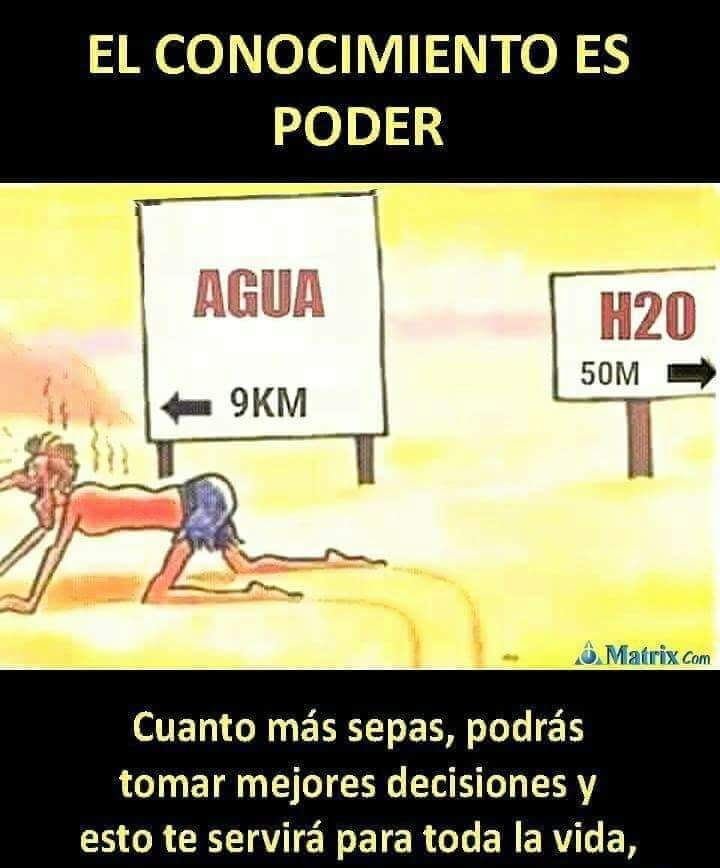
\includegraphics[width=.5\textwidth]{Conocimiento}
\end{figure}  
\end{frame}

\section{El problema de usar Google}
\begin{frame}
\begin{figure}
\centering
 
\includegraphics[width=.6\textwidth]{b1}
\end{figure}
\pause
Un problema de Google Académico es que los principiantes no son capaces de sacar provecho a todas sus capacidades.
\end{frame}



\begin{frame}
\begin{figure}
\centering
 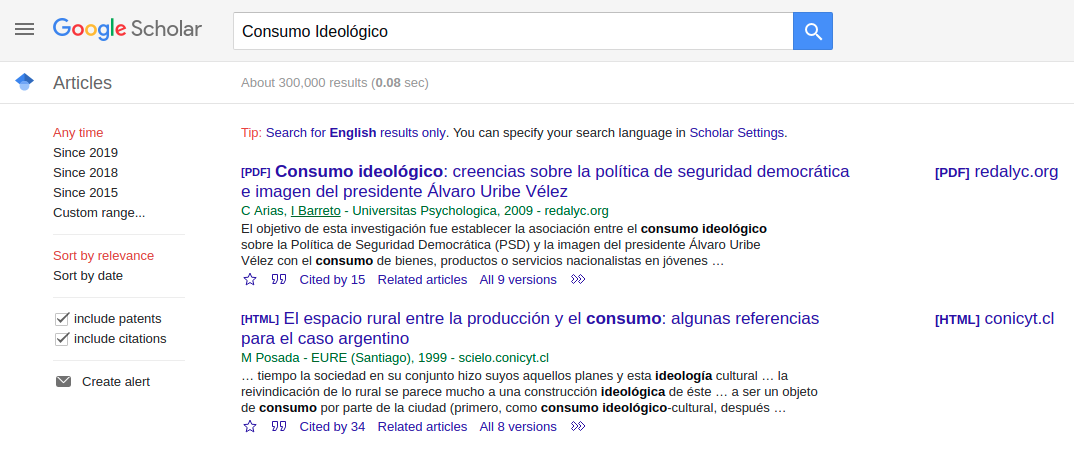
\includegraphics[width=1\textwidth]{b2}
\end{figure}
% \pause
Aquí los primeros dos resultados son del año 2009 y 1999 (i.e., referencias de hace 10 y 20 años respectivamente). También, se muestra cerca de 300 mil papers que cumplen con el criterio de búsqueda ``Consumo Ideológico''.\\
\pause
\vspace{0.3cm}
\textbf{¡Nadie va a leerse 300 mil papers para hacer su tesis!}
\end{frame}

\begin{frame}
\begin{figure}
\centering
 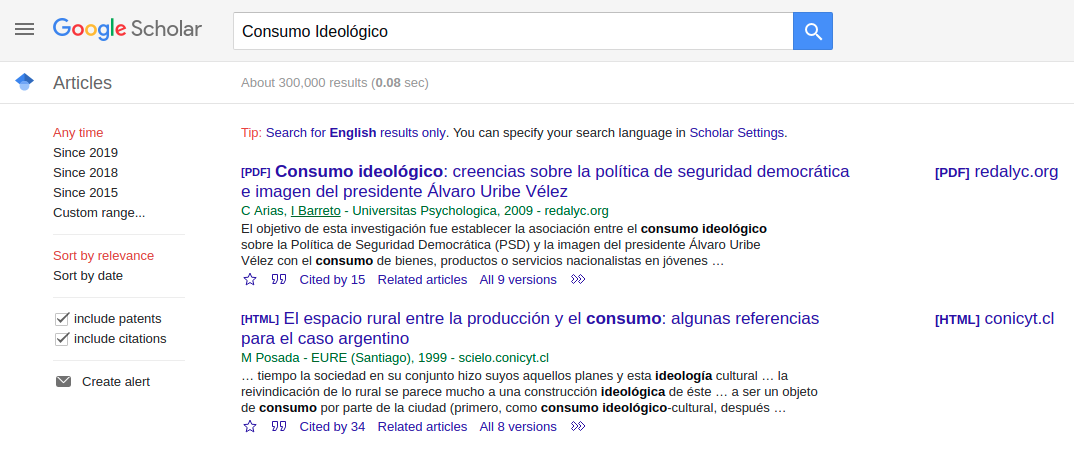
\includegraphics[width=.9\textwidth]{b2}
\end{figure}
Para el principiante tampoco es muy clara la decisión de cuál debe ser la primera referencia que se debería consultar o leer.
\end{frame}

\begin{frame}
\begin{figure}
\centering
 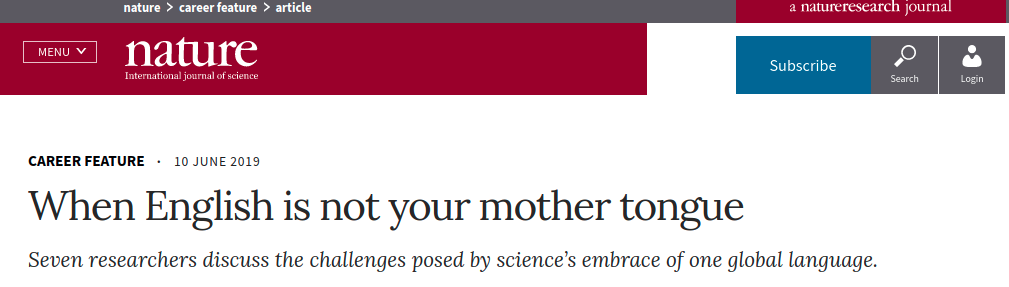
\includegraphics[width=.9\textwidth]{b3}
\end{figure}
\color{blue!46!green}
\url{https://www.nature.com/articles/d41586-019-01797-0}\\
\vspace{0.5cm}
\color{gray!72!black}
Para el principiante (cuya lengua materna no es el inglés) buscar en Español no es la estrategia más adecuada.
\end{frame}
    
\section{Estrategia 1 (Papers)}
\begin{frame}{Primera Estrategia de Búsqueda: El paper}
El conocimiento científico se organiza de forma jerárquica
\begin{figure}
\centering
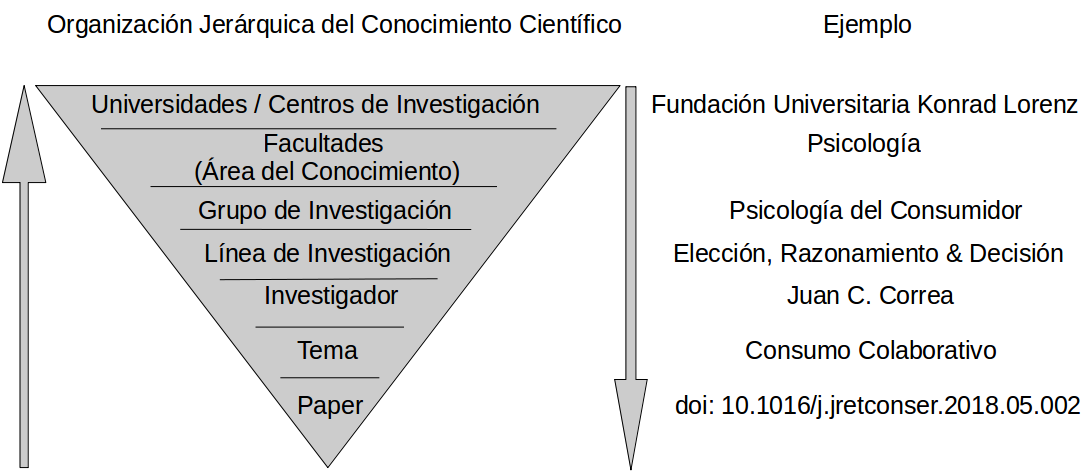
\includegraphics[width=.9\textwidth]{b4}
\end{figure}
Una búsqueda exitosa es aquella que da como resultado un conjunto de trabajos (papers) que abordan específicamente lo que uno quiere conocer.
\end{frame}

\begin{frame}{Primera Estrategia de Búsqueda: El paper}
Si estamos por iniciar un proceso de investigación, a veces puede ser efectiva la estrategia de comenzar a leer los libros técnicos.
\begin{figure}
\centering
 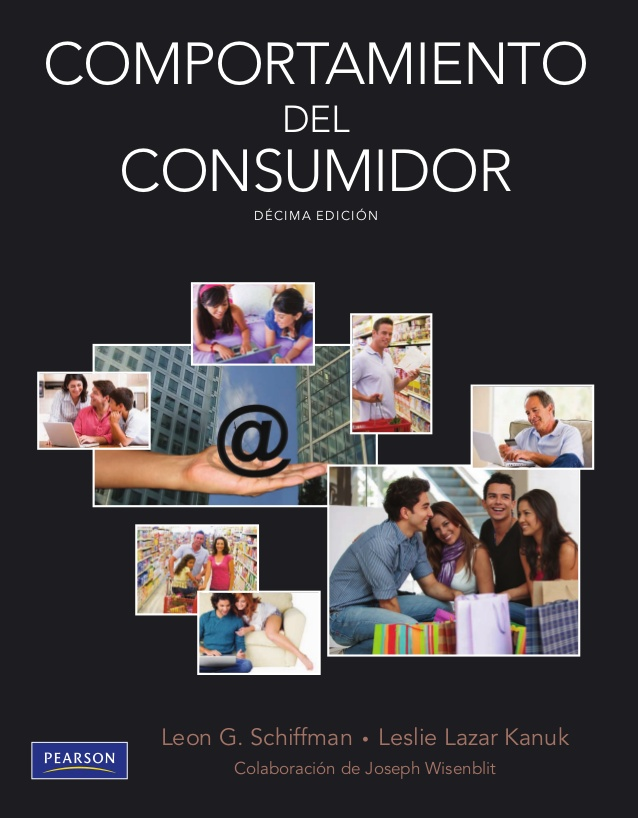
\includegraphics[width=.4\textwidth]{b5}
\end{figure}
\end{frame}

\begin{frame}{Primera Estrategia de Búsqueda: El paper}
Sin embargo, los libros técnicos son como ``colecciones'' de papers.
\begin{figure}
\centering
 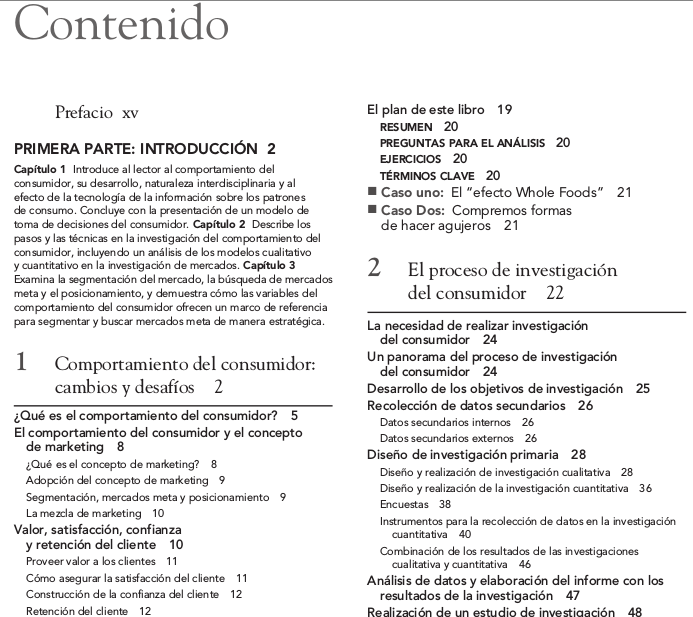
\includegraphics[width=.4\textwidth]{b6}
\end{figure}
Por un lado, los procesos editoriales de publicación de un libro son más largos que los procesos editoriales de publicar un paper. Por otro lado, los libros técnicos tienden a ser más costosos que los papers y no siempre hay libros técnicos específicos para un tema y cuando se consiguen, puede que sus contenidos ya estén desactualizados u obsoletos.
\end{frame}


\section{Estrategia 2 (Revistas)}
\begin{frame}{Segunda Estrategia de Búsqueda: Las Revistas (Journals)}
Las revistas son el medio de divulgación por excelencia del conocimiento científico cuya unidad mínima informativa es el paper.
\begin{figure}
\centering
 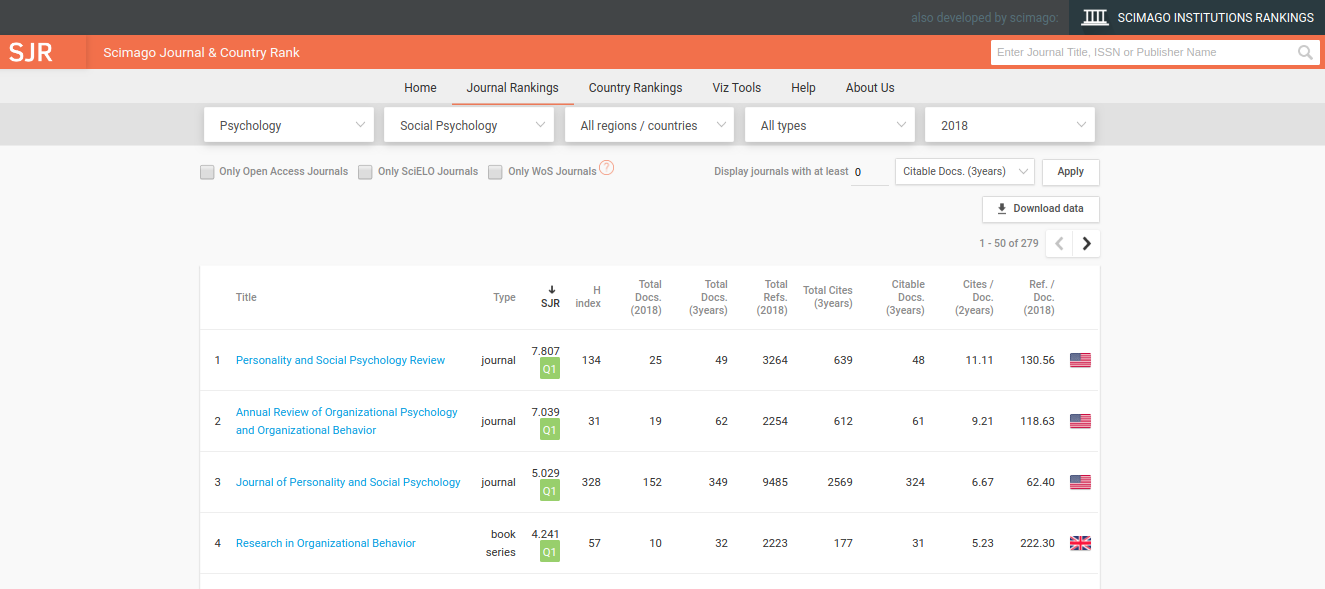
\includegraphics[width=1\textwidth]{b7}
\end{figure}
\color{blue!46!green}
\url{https://www.scimagojr.com/journalrank.php}
\end{frame}

\begin{frame}{Segunda Estrategia de Búsqueda: Las Revistas (Journals)}
Las revistas tienen nombres que, por lo general, revelan el tipo de conocimiento específico en el que se concentran sus publicaciones.
\begin{figure}
\centering
 
\includegraphics[width=0.8\textwidth]{b8}
\end{figure}
\end{frame}

\begin{frame}{Segunda Estrategia de Búsqueda: Las Revistas (Journals)}
Las revistas (al igual que los equipos de fútbol) tienen sus rankings. Hay revistas más prestigiosas y hay revistas de menor prestigio.
\begin{figure}
\centering
 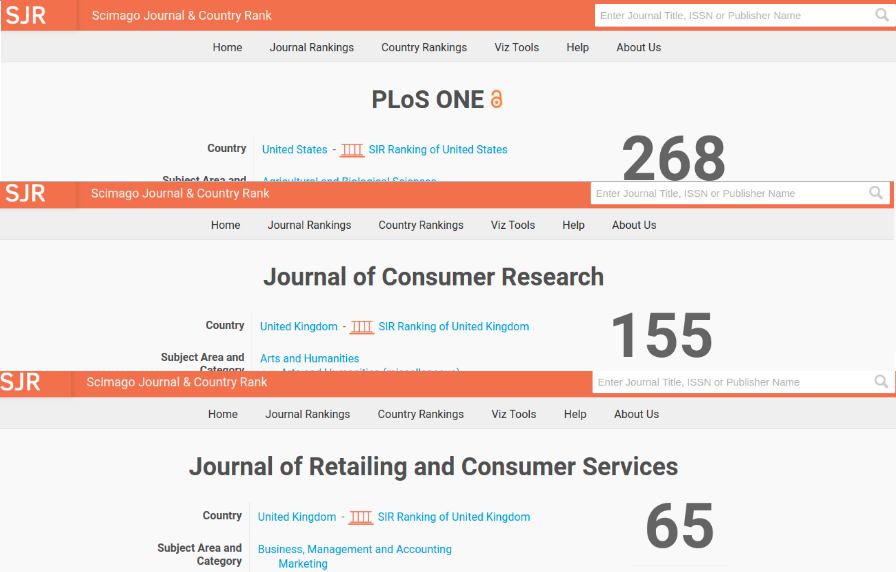
\includegraphics[width=0.8\textwidth]{b11}
\end{figure}
\end{frame}



\section{Estrategia 3 (Investigadores)}
\begin{frame}{Tercera Estrategia de Búsqueda: Los Investigadores}
Los investigadores son las personas que llevan a cabo una investigación según sus intereses académicos y la publican en la revista técnica de mayor relevancia para su disciplina.
\begin{figure}
\centering
 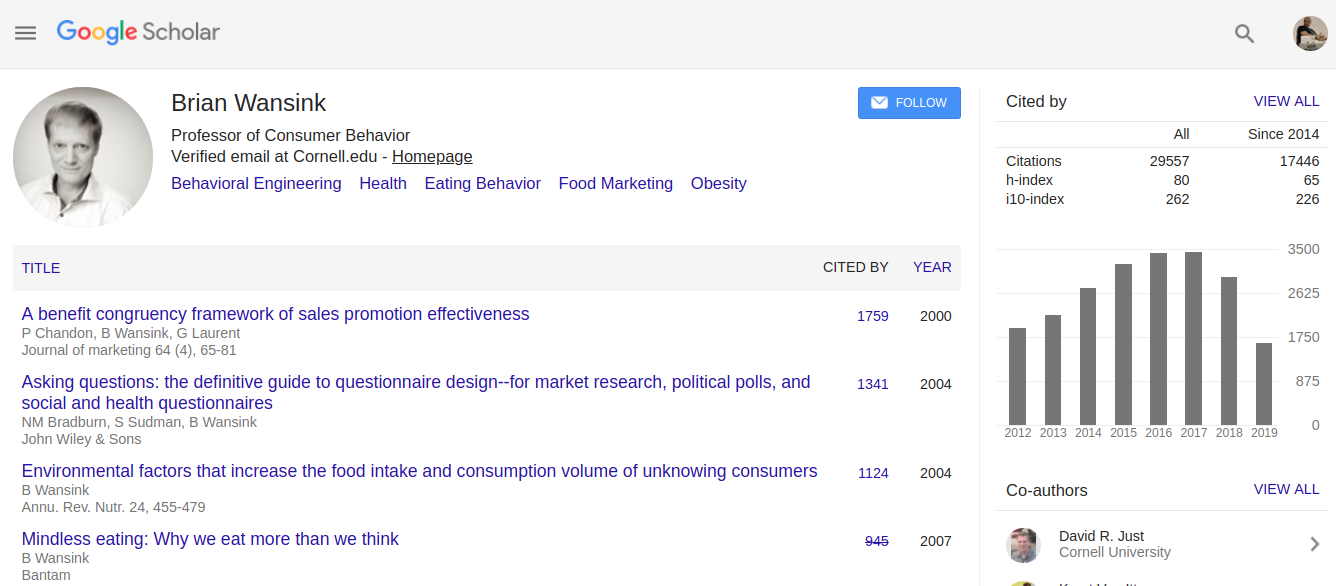
\includegraphics[width=1\textwidth]{b9}
\end{figure}
Si usted se sabe el nombre completo del investigador, puede buscarlo en Google Scholar para mirar su historial de publicaciones. 
\end{frame}

\begin{frame}{Tercera Estrategia de Búsqueda: Los Investigadores}
También puede buscar el historial de publicaciones de un investigador en Researchgate
\begin{figure}
\centering
 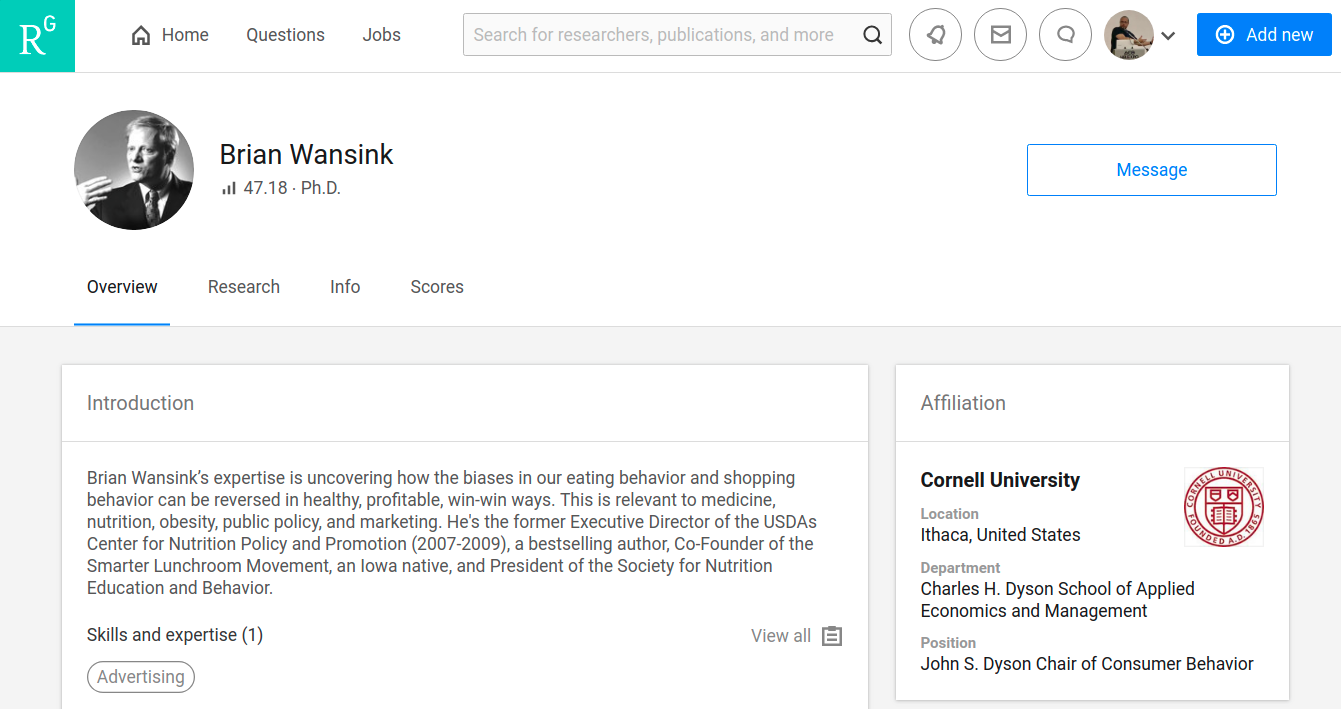
\includegraphics[width=1\textwidth]{b10}
\end{figure}
\color{blue!46!green}
\url{https://www.researchgate.net/}
\end{frame}

\begin{frame}{Tercera Estrategia de Búsqueda: Los Investigadores}
La trayectoria académica de un investigador se puede mirar por su H-Index, por el número de publicaciones que ha logrado, por las revistas en donde ha publicado, y por el tiempo (número de años) que lleva como investigador activo.
\begin{figure}
\centering
 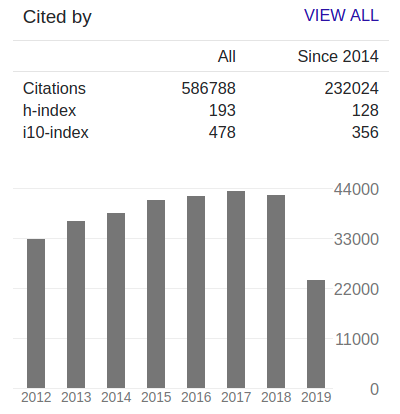
\includegraphics[width=0.3\textwidth]{b12}
\end{figure}
\end{frame}

\section{Sugerencias}
\begin{frame}{Recomendaciones para ser más eficientes en la búsqueda}
Si busca información para decidir el tema de una tesis, inicie buscando las publicaciones de sus docentes (Estrategia 3). 
\begin{figure}
\centering
 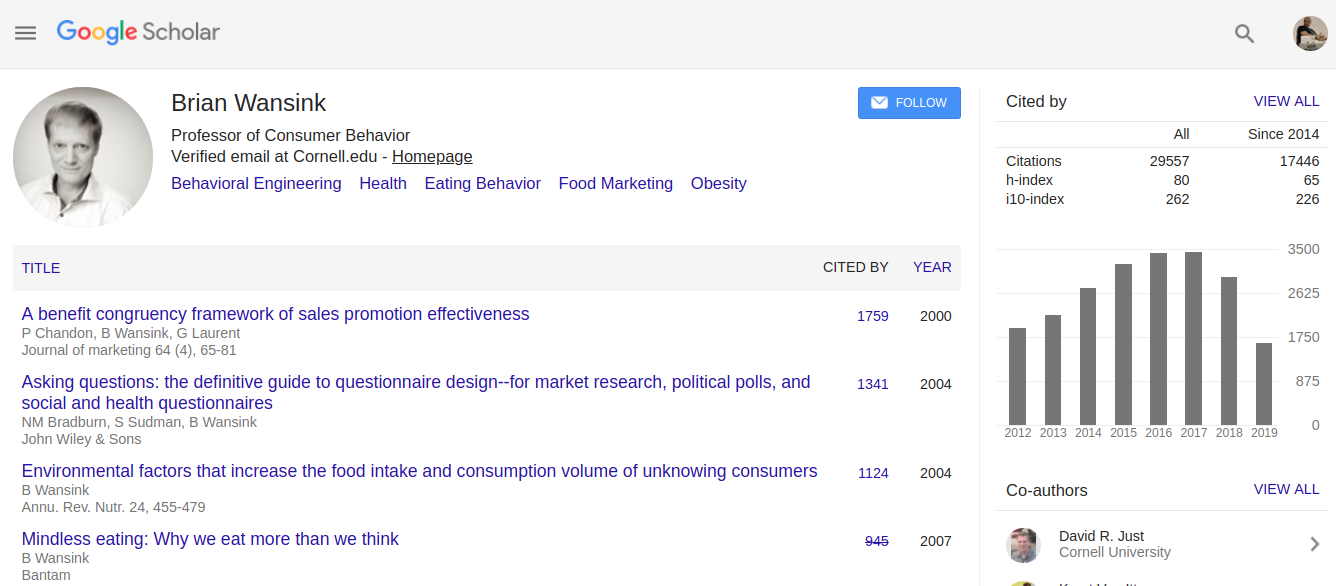
\includegraphics[width=0.8\textwidth]{b9}
\end{figure}
Averigue cuánto tiempo o dinero le llevó al investigador realizar sus investigaciones. Esta información usualmente se encuentra en la sección de ``materiales y métodos'' del paper.
\end{frame}

\begin{frame}{Tips para ser más eficientes en la búsqueda}
Si busca información para escribir un problema de investigación, haga búsquedas avanzadas en Scopus, combinando una palabra clave y una revista.
\begin{figure}
\centering
 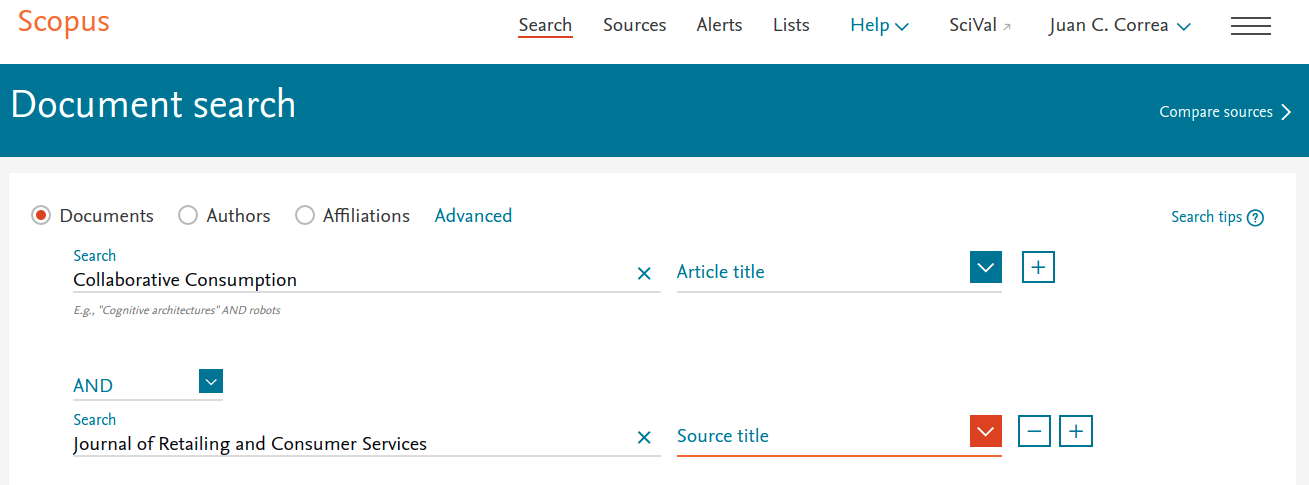
\includegraphics[width=1\textwidth]{b13}
\end{figure}
Aquí por ejemplo, se le está pidiendo a Scopus que nos devuelva la información de los papers que tengan las palabras ``Collaborative Consumption'' en su título, publicados específicamente en la revista ``Journal of Retailing and Consumer Services''.
\end{frame}

\begin{frame}{Tips para ser más eficientes en la búsqueda}
Como resultado de una búsqueda avanzada, lo ideal es obtener un número ``manejable'' de papers por leer (no más de 50).
\begin{figure}
\centering
 
\includegraphics[width=1\textwidth]{b14}
\end{figure}
En este caso, se ha obtenido como resultado únicamente tres papers que cumplen con el requerimiento específico que se mencionó en la lámina anterior.
\end{frame}

\begin{frame}{Tips para ser más eficientes en la búsqueda}
Descargue el pdf completo de cada paper encontrado. Suba el pdf a Mendeley Desktop, lea el abstract y las conclusiones de cada paper y apunte las ideas más relevantes en un documento de Word, usando la herramienta de ``Mendeley Cite-o-matic''.
\begin{figure}
\centering
 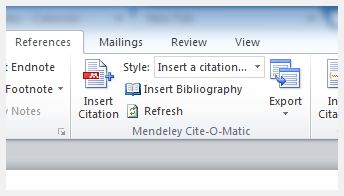
\includegraphics[width=.5\textwidth]{b15}
\end{figure}
Por ningún motivo separe la actividad de lectura de la escritura de ideas con sus citas. Aplique la técnica de \textbf{lea-escriba-cite}.
\end{frame}

\begin{frame}{Tips para ser más eficientes en la búsqueda}
Si no logra encontrar el pdf del paper, entonces recurra a las siguientes vías.
\begin{itemize}
    \item[1] Verifique si el pdf del paper se encuentra disponible en Researchgate o en los registros del perfil de Google Scholar
    \item[2] Escríbale un correo electrónico al autor para solicitarle amablemente una copia del pdf.
    \item[3] Use Facebook (Grupo BPPF) para pedirle el pdf en ese grupo. Pero primero lea las normas e instrucciones del grupo.
\end{itemize}
\end{frame}

\begin{frame}{Tips para ser más eficientes en la búsqueda}
Aprenda a usar Mendeley como un experto, para guardar sus archivos pdf, léerlos, hacer anotaciones y hacer citas bibliográficas con normas APA (\color{blue!46!green}\url{https://youtu.be/mLkO-aYzvx8}\color{gray!72!black}). Revise la bibliografía citada por cada paper que ya usted haya leído y aumente el número de papers conforme pasa el tiempo. 
\end{frame}

% \begin{frame}{Tips para ser más eficientes en la búsqueda}
% Inscríbase en el curso electivo de \textbf{``Introducción a Big Data''} para aprender a hacer bibliometrías de gran tamaño (revisión de miles o millones de papers), usando Bibliometrix. 
% \begin{figure}
% \centering
%  
\includegraphics[width=.3\textwidth]{b16}
% \end{figure}
% \color{blue!46!green}
% \url{https://youtu.be/V3vnYmfy0EI}
% \end{frame}





%\begin{frame}[allowframebreaks]{Referencias}
%\tiny{ 
%\bibliographystyle{apacite}
%\bibliography{references}
%} 
%\end{frame}

\end{document}